\label{sec:intro}
%Despite a lot of recent research, understanding the optimization and generalization for neural networks remain challenging problems: why can simple algorithm such as stochastic gradient descent optimize the complicated nonconvex objective, and why would the result generalize to unseen data? A common conjecture is that both problems are related to the loss landscape of neural networks. In this paper, we focus on an important aspect of the loss landscape \--- the layer-wise Hessian for neural networks along its training trajectory.

%Neural network objectives are complicated and non-convex. However, in practice neural networks can be trained by simple algorithms and they perform well on test data. A common explanation is that neural network objectives have good loss landscapes for optimization and generalization. In this paper we study the structure of Hessians for neural network objectives.

The loss landscape for neural networks is crucial for understanding training and generalization. In this paper we focus on the structure of Hessians, which capture important properties of the loss landscape. For optimization, Hessian information is used explicitly in second order algorithms, and even for gradient-based algorithms properties of the Hessian are often leveraged in analysis \citep{sra2012optimization}. For generalization, the Hessian captures the local structure of the loss function near a local minimum, which is believed to be related to generalization gaps \citep{keskar2016large}. %which is related to the intuition of flat vs. sharp local minimum, and can be incorporated into generalization bounds using ideas like PAC-Bayes bounds.

%Are the Hessians of neural networks similar to a random matrix or highly structured, and does the structure of Hessians change with different architecture or training algorithms? 
Several previous results including \citet{sagun2017empirical, papyan2018full} observed interesting structures in Hessians for neural networks \--- it often has around $c$ large eigenvalues where $c$ is the number of classes. In this paper we ask:
\begin{center}
    \emph{Why does the Hessian of neural networks have special structures in its top eigenspace?}
\end{center}

A rigorous analysis of the Hessian structure would potentially allow us to understand what the top eigenspace of the Hessian depends on (e.g., the weight matrices or data distribution), as well as predicting the behavior of the Hessian when the architecture changes. 

Towards this goal, we focus on the layer-wise Hessians in this paper. One difficulty in analyzing the layer-wise Hessian lies in its size \--- for a fully-connected layer with a $n\times n'$ weight matrix, the layer-wise Hessian is a $nn'\times nn'$ matrix. We propose a {\em decoupling conjecture} that approximates this matrix by the Kronecker product of two smaller matrices \--- a $n\times n$ input autocorrelation matrix and a $n'\times n'$ output Hessian matrix. We then study the properties of these two smaller matrices, which together with the decoupling conjecture give an explanation of why there are just a few large eigenvalues, as well as a heuristic formula to efficiently compute the top eigenspace. We prove the decoupling conjecture and structure of the output Hessian matrix for a simple model of 2-layer network. We then empirically verify that these results extend to much more general settings.



%Towards this goal, we first focus on the structure for the top {\em eigenspace} of layer-wise Hessians. %In this paper, we focus on the structures in the top eigenspace. 
%We observe that the top eigenspace of Hessians are far from random \--- models trained with different random initializations still have a large overlap in their top eigenspace, and the top eigenvectors are close to rank 1 when they are reshaped into the same shape as the corresponding weight matrix. 

%We formalize a conjecture that allows us to understand all these structures using a Kronecker decomposition. We also analyze the Hessian in an over-parametrized two-layer neural network for random data, proving that the output Hessian is approximately rank $c-1$ and its top eigenspace can be easily computed based on weight matrices.

%Towards rigorously proving the structures of Hessians for neural networks, we formalize a conjecture that allows us to understand the structures using a Kronecker decomposition. We also analyze the Hessian in an over-parametrized two-layer neural network for random data, proving that the Hessian is approximately rank $c-1$ and its top eigenspace can be easily computed based on weight matrices. The theoretical approach we take allows us to understand how the structures of the Hessian may depend on the choice of architecture or training algorithms \--- for example, it predicts that the structures become weaker when batch normalization is used (which was observed for top eigenvalue in \citet{ghorbani2019investigation}), or even just when the mean of each layer is set to 0. We also show that our new understanding can be leveraged to improve explicit generalization bounds similar to those in \citet{dziugaite2017computing}.


%What structures are there in the Hessian of neural network objectives?
%Previous works \citep{sagun2017empirical, papyan2018full} observed that the Hessian often has around $c$ large eigenvalues, where $c$ is the number of classes. In this paper we find more structure in the top eigenvectors and eigenspace of layer-wise Hessian. We can explain such structures by approximating the Hessian using a Kronecker decomposition. Our new understanding of the Hessian can be directly used to improve 
%We show that the eigenspaces of layer-wise Hessians also have other surprising behaviors: the top eigenspace of layer-wise Hessians from two randomly trained models have a high overlap at a dimension that is approximately equal to the layer's output-width; when the top eigenvectors of the layer-wise are viewed as matrices (with the same dimensions as the weight matrix), such matrices are approximately rank 1.

%We show that under a decoupling conjecture, one can approximate the layer-wise Hessian using the Kronecker product of the covariance of its input and its output Hessian. This Kronecker decomposition and the low rank properties of its two components allow us to explain the interesting properties of the layer-wise Hessians. Our explanation also shows that when batch normalization is enabled some of these properties no longer holds. 

%Better understanding of the Hessian can give more insights into optimization and generalization. As a directly application of our results, we show that the Hessian structure can be used to improve the PAC-Bayes bound computed in \citet{}; we also show that the general structure of the Hessian suggests a simple way of incorporating second-order information in optimization without large overhead.

%\rnote{Maybe make the above three paragraph even shorter?}

% \subsection{Our Results}
% \begin{figure}[th]
% \vspace{-6pt}
%     \centering
%     \begin{subfigure}[b]{0.58\textwidth}
%         \centering
%         \captionsetup{justification=centering}
%         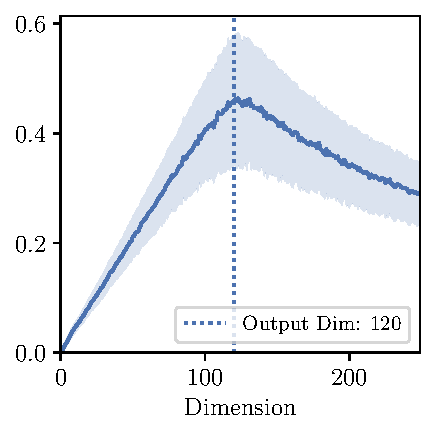
\includegraphics[width=0.45\textwidth]{Figures/SubspaceOverlap/NLeNet5_multi_hyperparam/DimOverlap_CIFAR10_LeNet5_normnew_fixlr0.001_X_LeNet5_normnew_fixlr0.01_X_LeNet5_normnew_fixlr0.01_momentum_fc1.pdf}
%         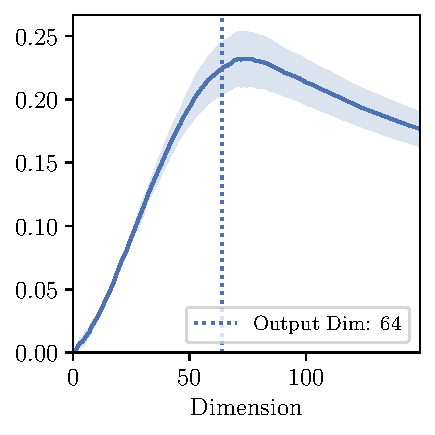
\includegraphics[width=0.45\textwidth]{Figures/SubspaceOverlap/ResNets/DimOverlap_CIFAR100_Resnet18W64New_nobn_fixlr0.01_layer3.0.conv2.pdf}
%         \caption{Overlap between dominate eigenspace of layer-wise Hessian at different minima for fc1:LeNet5 (\textbf{left}) with output dimension 120 and conv11:ResNet18-W64 (\textbf{right}) with output dimension 64.}
%         \label{fig:intro_overlap}
%     \end{subfigure}%
%     \begin{subfigure}[b]{0.38\textwidth}
%         \centering
%         \captionsetup{justification=centering}
%         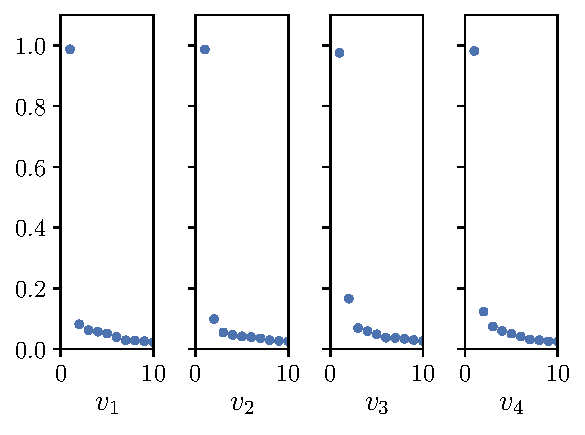
\includegraphics[width=0.9\textwidth]{Figures/Eigenvec_single/Top_Eigenvector_sigs_CIFAR10_Exp1_LeNet5_fixlr0.01R1_E-1fc1.pdf}
%         \caption{Top 10 singular values of the top 4\linebreak eigenvectors of the layer-wise Hessian of\linebreak fc1:LeNet5 after reshaped as matrix.}
%         \label{fig:intro_lowrank}
%     \end{subfigure}%
%     \caption{Some interesting observations on the structure of layer-wise Hessians.  The eigenspace overlap is defined in \definitionref{:overlap} and the reshape operation is defined in \definitionref{:matricization}}
%     \label{fig:intro_figs}
%     \vspace{-6pt}
% \end{figure}

\subsection{Outline}

\textbf{Understanding Hessian Structure using Kronecker Factorization:} %We show that both of these new properties of layer-wise Hessians can be explained by a Kronecker Factorization. 
In \sectionref{sec:hessian} We first formalize a decoupling conjecture that states  the layer-wise Hessian can be approximated by the Kronecker product of the output Hessian and input auto-correlation. 

The auto-correlation of the input is often very close to a rank 1 matrix, because the inputs for most layers have a nonzero expectation. We show that when the input auto-correlation component is approximately rank 1, top eigenspace of the layerwise Hessian is very similar to that of the output Hessian. %the layer-wise Hessians indeed have high overlap at the dimension of the layer's output, and the spectrum of the layer-wise Hessian is similar to the spectrum of the output Hessian. 
On the contrary, when inputs have mean 0 (e.g., when the model is trained with batch normalization), the input auto-correlation matrix is much farther from rank 1 and the layer-wise Hessian often does not have the same low rank structure.

In \sectionref{sec:theoretical} we prove that in an over-parametrized two-layer neural network on random data, the output Hessian is approximately rank $c-1$. Further, we can compute the top $c-1$ eigenspace directly from weight matrices. We show a similar low rank result for %can also prove the decoupling conjecture in this setting, showing that 
the layer-wise Hessian. % is indeed low rank.


%This Kronecker approximation directly implies that the eigenvectors of the layer-wise Hessian should be approximately rank 1 when viewed as a matrix. Moreover, under stronger assumptions, we can generalize the approximation for the top eigenvalues and eigenvectors of the full Hessian.

\textbf{Implication on the Structure of Top Eigenspace for Hessians:} The decoupling conjecture, together with our characterizations of its two components, have surprising implications to the structure of top-eigenspace for layer-wise Hessians. Since the eigenvector of a Kronecker product is just the outer product of eigenvectors of its components, if we express the top eigenvectors of a layer-wise Hessian as a matrix with the same dimensions as the weight matrix, then the matrix is approximately rank 1. In \figureref{fig:intro_figs}.a we show the singular values of several such reshaped eigenvectors. Another more surprising phenomenon considers the overlap between top eigenspaces for different models.

% \begin{figure}[th]
% \vspace{-6pt}
%     \centering
% \captionsetup[sub]{format=subcaptionformat}
%     \begin{subfigure}[b]{0.58\textwidth}
%         \centering
%         \captionsetup{justification=centering}
%         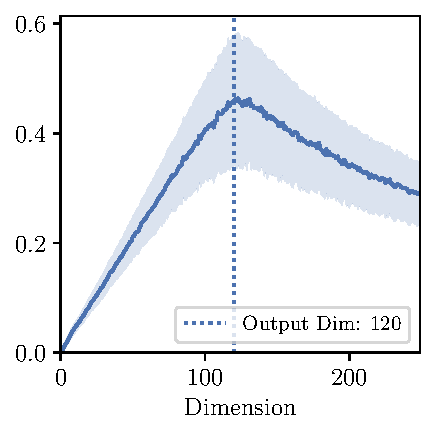
\includegraphics[width=0.45\textwidth]{Figures/SubspaceOverlap/NLeNet5_multi_hyperparam/DimOverlap_CIFAR10_LeNet5_normnew_fixlr0.001_X_LeNet5_normnew_fixlr0.01_X_LeNet5_normnew_fixlr0.01_momentum_fc1.pdf}
%         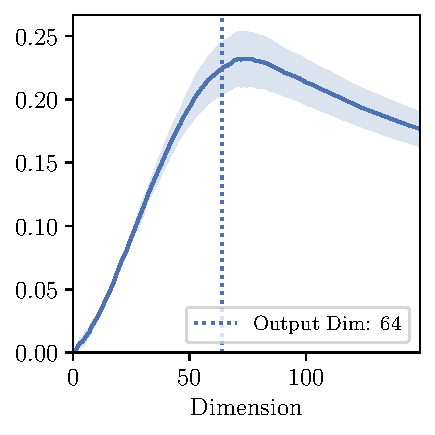
\includegraphics[width=0.45\textwidth]{Figures/SubspaceOverlap/ResNets/DimOverlap_CIFAR100_Resnet18W64New_nobn_fixlr0.01_layer3.0.conv2.pdf}
%         \caption{Overlap between dominate eigenspace of layer-wise Hessian at different minima for fc1:LeNet5 (\textbf{left}) with output dimension 120 and conv11:ResNet18-W64 (\textbf{right}) with output dimension 64.}
%         \label{fig:intro_overlap}
%     \end{subfigure}%
%     \begin{subfigure}[b]{0.38\textwidth}
%         \centering
%         \captionsetup{justification=centering}
%         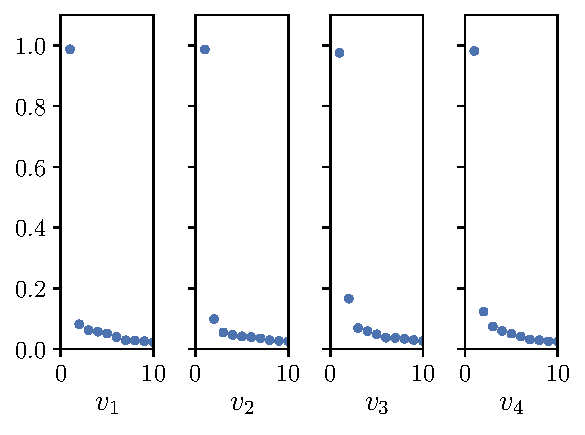
\includegraphics[width=0.9\textwidth]{Figures/Eigenvec_single/Top_Eigenvector_sigs_CIFAR10_Exp1_LeNet5_fixlr0.01R1_E-1fc1.pdf}
%         \caption{Top 10 singular values of the top 4\linebreak eigenvectors of the layer-wise Hessian of\linebreak fc1:LeNet5 after reshaped as matrix.}
%         \label{fig:intro_lowrank}
%     \end{subfigure}%
%     \caption{Some interesting observations on the structure of layer-wise Hessians.  The eigenspace overlap is defined in \cref{def:overlap} and the reshape operation is defined in \cref{def:matricization}}
%     \label{fig:intro_figs}
%     \vspace{-6pt}
% \end{figure}
\begin{figure}[th]
\vspace{-6pt}
    \centering
\captionsetup[sub]{format=subcaptionformat}
    \begin{subfigure}[b]{0.58\textwidth}
        \centering
        \captionsetup{justification=centering}
        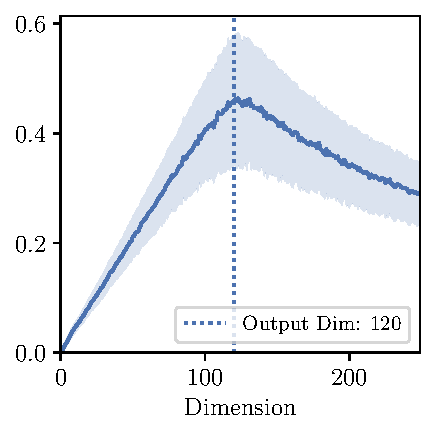
\includegraphics[width=0.45\textwidth]{Figures/SubspaceOverlap/NLeNet5_multi_hyperparam/DimOverlap_CIFAR10_LeNet5_normnew_fixlr0.001_X_LeNet5_normnew_fixlr0.01_X_LeNet5_normnew_fixlr0.01_momentum_fc1.pdf}
        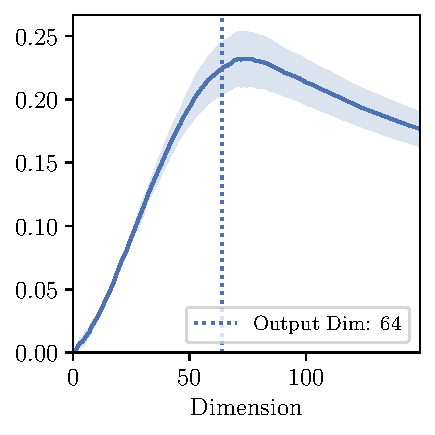
\includegraphics[width=0.45\textwidth]{Figures/SubspaceOverlap/ResNets/DimOverlap_CIFAR100_Resnet18W64New_nobn_fixlr0.01_layer3.0.conv2.pdf}
        \caption{Overlap between dominate eigenspace of layer-wise Hessian at different minima for fc1:LeNet5 (\textbf{left}) with output dimension 120 and conv11:ResNet18-W64 (\textbf{right}) with output dimension 64.}
        \label{fig:intro_overlap}
    \end{subfigure}%
    \begin{subfigure}[b]{0.38\textwidth}
        \centering
        \captionsetup{justification=centering}
        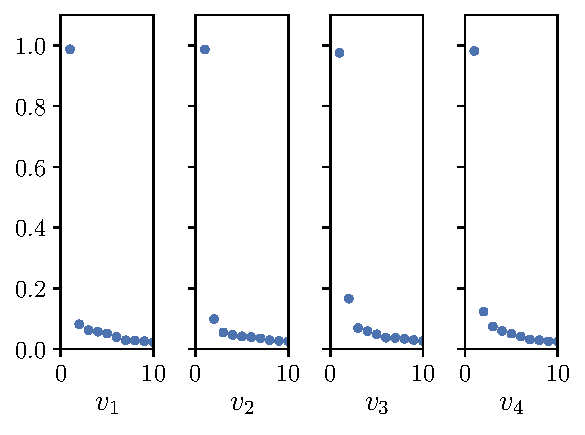
\includegraphics[width=0.9\textwidth]{Figures/Eigenvec_single/Top_Eigenvector_sigs_CIFAR10_Exp1_LeNet5_fixlr0.01R1_E-1fc1.pdf}
        \caption{Top 10 singular values of the top 4\linebreak eigenvectors of the layer-wise Hessian of\linebreak fc1:LeNet5 after reshaped as matrix.}
        \label{fig:intro_lowrank}
    \end{subfigure}%
    \caption{Some interesting observations on the structure of layer-wise Hessians.  The eigenspace overlap is defined in \cref{def:overlap} and the reshape operation is defined in \cref{def:matricization}}
    \label{fig:intro_figs}
    \vspace{-6pt}
\end{figure}
Consider two neural networks trained with different random initializations and potentially different hyper-parameters; their weights are usually nearly orthogonal. One might expect that the top eigenspace of their layer-wise Hessians are also very different. However, empirically one observe that the top eigenspace of the layer-wise Hessians have a very high overlap, and the overlap peaks at the dimension of the layer's output (see \figureref{fig:intro_overlap}). This is a direct consequence of the Kronecker product and the fact that the input auto-correlation matrix is close to rank 1.




%\znote{Added some content regarding the full hessian approximation}


%\textbf{Leveraging Hessian Structure:}
%Better understanding of the Hessian can give more insights into optimization and generalization. 
\textbf{Applications:} As a direct application of our results, in \sectionref{sec:pac} we show that the Hessian structure can be used to improve the PAC-Bayes bound computed in \citet{dziugaite2017computing}. %; we also show that the general structure of the Hessian suggests a simple way of incorporating second-order information in optimization without large overhead.

